\documentclass[aspectratio=169]{beamer}

% arara: pdflatex 
% arara: biber
% arara: pdflatex
% arara: pdflatex
% arara: clean: {extensions: [aux, bbl, out, toc, blg, thm, log, bcf, snm, nav]}

\usetheme[lightmode, showmaxslides]{pureminimalistic} %darkmode vs lightmode

% *****************************************************************
% Classic
% *****************************************************************
\usepackage[english]{babel}
\usepackage[utf8]{inputenc}
\usepackage[T1]{fontenc}
\usepackage{hyperref}


% ********** Basic supplementray materials
% \usepackage{hvfloat}  % rotation of caption
% \usepackage{rotating}  % allow complete rotation
\usepackage{soul}  % strikethrough text
\usepackage[normalem]{ulem}  % underline text
\usepackage{xcolor}  % color 
% **********


% ********** Maths packages
\usepackage{amssymb,amsmath}
\usepackage{graphicx}
% \usepackage{tikz}
% **********


% ********** Table packages
\usepackage{array}
\usepackage{booktabs}
\usepackage{colortbl}  % color cells
% \usepackage{longtable}
\usepackage{siunitx}
% \usepackage{tabu}
% \usepackage{threeparttable} 
% **********


% ********** Icones packages
\usepackage{fontawesome}
\usepackage{orcidlink}
\usepackage{tfrupee}
% **********


% ********** Define color + color configuration
\definecolor{NUred}{RGB}{213, 17, 45}
\definecolor{NUblue}{RGB}{0, 59, 113}
\definecolor{UBbrown}{RGB}{48, 33, 25}
\definecolor{UBblue}{RGB}{0, 158, 214}
\definecolor{ODRIISdarkgreen}{RGB}{80,151,68}
\definecolor{ODRIISlightgreen}{RGB}{164,204,76}
\definecolor{ODRIISbrick}{RGB}{197,102,63}
\definecolor{lightgray}{HTML}{A9A9A9}
\definecolor{lightgray2}{RGB}{113,113,113}
% **********
\hypersetup{colorlinks,linkcolor={lightgray2},citecolor={ODRIISdarkgreen},urlcolor={ODRIISdarkgreen}}
%\renewcommand{\beamertextcolor}{}
%\renewcommand{\beamerbgcolor}{}
%\renewcommand{\beamerfootertextcolor}{}
\renewcommand{\beamertitlecolor}{ODRIISbrick}
\setbeamercolor{button}{bg=ODRIISdarkgreen,fg=ODRIISlightgreen!10}
% **********





% *****************************************************************
% Pureminimalistic configuration
% *****************************************************************
\renewcommand{\logotitle}{\vspace*{-20mm}\hspace*{-10.1mm}
\includegraphics[width=\paperwidth]{Beamer_theme/header2.jpeg}}
\renewcommand{\logoheader}{\vspace{0em}}
\renewcommand{\logoheader}{\vspace{0em}}
\renewcommand{\logofooter}{\href{https://odriis.hypotheses.org/}{
\includegraphics[width=.6\linewidth]{Beamer_theme/odriis_long.png}}}



% *****************************************************************
% Caption configuration
% *****************************************************************
\usepackage{caption}  % custom caption

\captionsetup{
font=small,
skip=1em,
labelfont={bf},
justification=centering,
singlelinecheck=false,
%textfont={bf,it},
%labelsep=endash,
%tableposition=top,
}






% *****************************************************************
% Appendix
% *****************************************************************
\usepackage{appendixnumberbeamer}
\renewcommand{\appendixname}{\texorpdfstring{\translate{appendix}}{appendix}}





% *****************************************************************
% Bibliography
% *****************************************************************

% ********** Bibtex
% \usepackage[doi, natbibapa]{apacite}
% \renewcommand\bibliographytypesize{\tiny}
% \let\realcitep\citep
% \renewcommand*{\citep}[1]{{\small\realcitep{#1}}}
% \let\realcite\cite
% \renewcommand*{\cite}[1]{{\small\realcite{#1}}}
% ********** 


% ********** Biblatex
\usepackage[
natbib=true,
backend=biber,
style=trad-abbrv,
sorting=none, %nyt
]{biblatex}
% **********
\renewcommand*{\bibfont}{\footnotesize}





% *****************************************************************
% Bigcenter
% *****************************************************************
\makeatletter
\newskip\@bigflushglue \@bigflushglue = -100pt plus 1fil
\def\bigcenter{\trivlist \bigcentering\item\relax}
\def\bigcentering{\let\\\@centercr\rightskip\@bigflushglue%
\leftskip\@bigflushglue
\parindent\z@\parfillskip\z@skip}
\def\endbigcenter{\endtrivlist}
\makeatother






% *****************************************************************
% Box creation
% *****************************************************************
\usepackage[most]{tcolorbox}

\newtcolorbox{greenbox}[2][]{colback=ODRIISlightgreen!10,colframe=ODRIISlightgreen!10,coltitle=black,colbacktitle=ODRIISdarkgreen!20,title={#2},#1}
\newtcolorbox{brickbox}[1][]{colback=ODRIISbrick!10,colframe=ODRIISbrick!10,#1}






% *****************************************************************
% Section page
% *****************************************************************
\newcommand{\secttitle}[1]{
\begin{columns} 
\begin{column}{.4\textwidth}
\vspace*{-0mm}\hspace*{-10.1mm}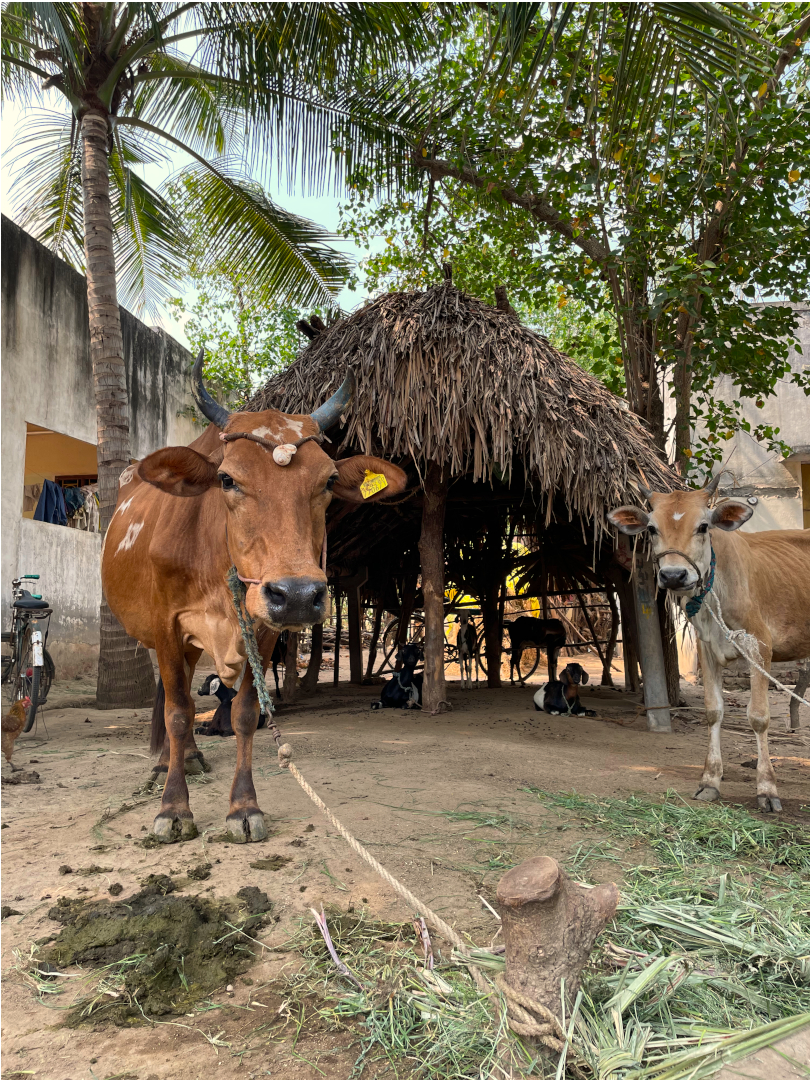
\includegraphics[height=\paperheight]{Beamer_theme/cow.jpeg}
\end{column}
\begin{column}{.6\textwidth}
\vfill
\begin{tcolorbox}[colback=ODRIISlightgreen!20,colframe=ODRIISlightgreen!20,box align=center,halign=center,valign=center]
{\LARGE \textcolor{ODRIISbrick}{#1}}
\end{tcolorbox}
\vfill
\end{column}
\end{columns}
}






% *****************************************************************
% Table
% *****************************************************************

% ********** Stars
\newcommand{\sym}[1]{\rlap{#1}}% Thanks to David Carlisle
% **********


% ********** Insert the table
\newcommand{\inserttable}[3]{
\resizebox{#3}{!}{
\begin{tabular}{#2}
\toprule
\input #1
\bottomrule
\end{tabular}
}
}
% **********


% ********** Source
\newcommand{\bottomtext}[1]{\vspace{-1.5ex}\captionsetup{justification=centering,font=footnotesize,singlelinecheck=false}\caption*{\hangindent=1.5em #1}}
\newcommand{\bottomnote}[1]{\bottomtext{\textit{Note}:~#1}}
\newcommand{\source}[1]{\bottomtext{\textit{Source}:~#1}}
\newcommand{\starnote}{\bottomtext{* p < 0.1, ** p < 0.05, *** p < 0.01. Standard error in parentheses.}}
% **********


% ********** siunitx config
\sisetup{
detect-mode,
tight-spacing= true,
group-digits= false ,
input-signs= ,
input-symbols= ( ) [ ] - + *,
input-open-uncertainty=,
input-close-uncertainty=,
table-align-text-post=false
}
% **********


% ********** Linebreak in cell
\newcommand{\specialcell}[2][c]{\begin{tabular}[#1]{@{}c@{}}#2\end{tabular}}
% **********


% \makeatletter
% \AddToHook{env/tabular/begin}{\let\input\@@input}
% \makeatother




% *****************************************************************
% Personnal cmd
% *****************************************************************
\newcommand{\jati}[1]{\textit{j\={a}ti{#1}}}

\newcommand\dev[1]{\textbf{\textcolor{red}{#1}}}

\newcommand{\ie}{i.e.}
\newcommand{\sd}{standard deviation}
\newcommand{\pp}{percentage points}
\newcommand{\aebe}{all else being equal}
\newcommand{\Aebe}{All else being equal}
\newcommand{\ote}{other things equal}
\newcommand{\Ote}{Other things equal}
\newcommand{\cl}{confidence level}
\newcommand{\lit}{\dev{literature}}
\newcommand{\PTCS}{PT\&CS}

\newcommand{\key}[1]{\underline{\textsc{#1}}}
\newcommand{\data}[1]{\textbf{\underline{Data #1:}}~}


% ********** Symbol shortcuts
\def\@fnsymbol#1{\ensuremath{\ifcase#1\or *\or \dagger\or \ddagger\or
   \mathsection\or \mathparagraph\or \|\or **\or \dagger\dagger
   \or \ddagger\ddagger \else\@ctrerr\fi}}
   
\makeatletter
\newcommand{\ssymbol}[1]{^{\@fnsymbol{#1}}}
\makeatother
% **********

% ********** Bibliography
\addbibresource{Ref_Arnaud.bib}
% ********** 

\setbeamercovered{transparent}






% *****************************************************************
% Title
% *****************************************************************
\title[Psychology of debt]{\textsc{Psychology of Debt in Rural South India}}
\author[A. Natal and C.J. Nordman]{\textcolor{ODRIISdarkgreen}{Arnaud Natal\orcidlink{0000-0003-1301-2281}} \textcolor{ODRIISlightgreen}{\scriptsize Univ. Bordeaux} \\ 
\textcolor{ODRIISdarkgreen}{Christophe J. Nordman} \textcolor{ODRIISlightgreen}{\scriptsize LEDa-DIAL, IRD, PSL University and IFP}} 
\institute{\\ ICDE | \small \today} 


% ******************************************************************
\begin{document}

\maketitle



% *******************
\begin{frame}{Motivation}
Increasing interest in:
\begin{itemize}
	\item Personality traits and cognitive skills (\PTCS~) \citep{Almlund2011};
	\item Household finance.
	\item[$\rightarrow$] in the USA;
	\item[$\rightarrow$] in the UK.
\end{itemize}

Developping countries remains a blind spot, while:
\begin{enumerate}
	\item Credit as exit to poverty;
	\item Informal debt.
\end{enumerate}

\begin{brickbox}
\centering Fill this gap by considering the case of rural South India.
\end{brickbox}

\end{frame}
% *******************



% *******************
\begin{frame}[plain,noframenumbering]

\secttitle{Theoretical framework}

\end{frame}
% *******************




% *******************
\begin{frame}{Theoretical framework I}

Increasing of debt in rural India since the 1980's:
\begin{itemize}
\item Incidence goes from 19 to 32\%, 
\item but largely underestimated: 80-90\%.
\item Amount goes from 283 to 33,000.
\item[$\rightarrow$] Good debt management is essential.% and literature highlights individual psychology in debt management \citep{Amar2011}.
\end{itemize}


Especially to the disadvantage of \textit{Dalits}, and females.

%Recent crises are fuelling this increase and widening inequalities \citep{GuerinDemo2017,Guerin2022}.
\begin{itemize}
\item[$\rightarrow$] Need to take into account the social identity.
\end{itemize}

\end{frame}
% *******************




% *******************
\begin{frame}{Theoretical framework II}

The cornerstone of debt in India is its social meaning
\begin{itemize}
\item Set of rights and obligations that links borrowers (Br) and lenders (Lr) into a strong relationship.
\item Consequences in terms of social belonging, status, and dignity.
\item Not fixed but continuously bargained and negotiated.
\item[$\rightarrow$] Expression of individual differences in the negotiation process.
\end{itemize}

\end{frame}
% *******************






% *******************
\begin{frame}[plain,noframenumbering]

\secttitle{Data \& methodology}

\end{frame}
% *******************






% *******************
\begin{frame}{Empirical strategy II}
To take into account the weight of social identity, we use interaction variables:

\begin{align}
\label{eq:reg2} Y_{i} & = \beta_{0}+PTCS'_{i}*\beta_{1}+X'_{i}*\beta_{2}+PTCS'_{i}*Sex_{i}*\beta_{3}+\epsilon_i  \\ 
\label{eq:reg3} Y_{i} & = \beta_{0}+PTCS'_{i}*\beta_{1}+X'_{i}*\beta_{2}+PTCS'_{i}*Caste_{i}*\beta_{3}+\epsilon_i  \\ 
\label{eq:reg4} Y_{i} & = \beta_{0}+PTCS'_{i}*\beta_{1}+X'_{i}*\beta_{2}+PTCS'_{i}*Sex_{i}*Caste_{i}*\beta_{3}+\epsilon_i 
\end{align}

\begin{greenbox}{Interpretation}
ME at representative values of sex and caste.
All other covariables at the mean. 
Allows us to create 9 subgroups of ME. 
\begin{itemize}
\item[$\rightarrow$] How the effects of \PTCS~ vary according to social identities?
\end{itemize}
\end{greenbox}

\end{frame}
% *******************







% *******************
\begin{frame}[plain,noframenumbering]

\secttitle{Descriptive statistics}

\end{frame}
% *******************





% *******************
\begin{frame}{Household level statistics IV}

% \begin{figure}[h]
% \centering
% \includegraphics[scale=0.7]{INPUT/Kernel_PTCS}
% \source{NEEMSIS-1 (2016-17); author's calculations.}
% \end{figure}


\end{frame}
% *******************












% *******************
\section*{References}
\begin{frame}[noframenumbering, allowframebreaks]{References}

\printbibliography[title={References},heading=none]

\end{frame}
% *******************









% *******************
\begin{frame}[noframenumbering]{Contacts}
 
\begin{columns}
\begin{column}{0.5\textwidth}
\begin{center}
Arnaud Natal, \\
\textcolor{ODRIISlightgreen}{\footnotesize{Univ. Bordeaux, CNRS, BSE, UMR 6060}} \\
\href{https://orcid.org/0000-0003-1301-2281}{\footnotesize{orcid.org/0000-0003-1301-2281}} \\
\href{mailto:arnaud.natal@u-bordeaux.fr}{\footnotesize{arnaud.natal@u-bordeaux.fr}} \\
\href{https://arnaudnatal.github.io}{\footnotesize{arnaudnatal.github.io}}
\end{center}
\end{column}
\begin{column}{0.5\textwidth}  %%<--- here
\begin{center}
Christophe J. Nordman, \\
\textcolor{ODRIISlightgreen}{\footnotesize{LEDa-DIAL, IRD, PSL University and IFP}}
\href{mailto:nordman@dial.prd.fr}{\footnotesize{nordman@dial.prd.fr}} \\
\end{center}
\end{column}
\end{columns}


\vskip0ptplus1filll\relax
\begin{center}
\small Credit images: BTS. April 27, 2021. Manam.
\end{center}

\end{frame}
% *******************





\end{document}





% *******************
%\begin{frame}[plain, shrink=2]{Correction 1 \citep{Rammstedt2013}}
%\begin{figure}[htpb]
%\centering
%\includegraphics[scale=1]{INPUT/boxplotars.pdf}
%\end{figure}
%\end{frame}
% *******************





% *******************
%\begin{frame}[plain, shrink=2]{Résultats}
%\input{INPUT/AME_indebt.tex}
%\end{frame}
% *******************

% *******************
% \begin{frame}{Figures}
%     \begin{figure}[H]
%         \centering
%         \begin{columns}[T]
%             \begin{column}{.3\linewidth}
%                 \includegraphics[width=\linewidth]{example-image-a}
%                 \caption{Example A}
%             \end{column}
%             \begin{column}{.3\linewidth}
%                 \includegraphics[width=\linewidth]{example-image-b}
%                 \caption{Example B}
%             \end{column}
%         \end{columns}
%     \end{figure}
% \end{frame}
% *******************